\chapter{Hashing}
Nei capitoli precedenti abbiamo affrontato il concetto di \nameref{def:29} e
abbiamo visto come la scelta della \emph{struttura dati} si ripercuota sulla
\emph{complessità} delle operazioni.

In particolare, abbiamo osservato le seguenti \emph{complessità}:

\begin{table}[h]
    \renewcommand{\arraystretch}{1.2}
    \centering
    \begin{tabular}{|c|c|c|c|c|c|}
        \hline
        \textbf{Operazione} & \textbf{Array non ordinato} & \textbf{Array ordinato}
        & \textbf{Lista} & \textbf{Alberi RB}\\
        \hline
        \texttt{insert()} & $O(1),\,O(n)$ & $O(n)$ & $O(1),\,O(n)$ & $O(\log n)$\\
        \hline
        \texttt{lookup()} & $O(n)$ & $O(\log n)$ & $O(n)$ & $O(\log n)$\\
        \hline
        \texttt{remove()} & $O(n)$ & $O(n)$ & $O(n)$ & $O(\log n)$\\
        \hline
        \texttt{foreach} & $O(n)$ & $O(n)$ & $O(n)$ & $O(n)$\\
        \hline
    \end{tabular}
\end{table}\noindent
Esiste una \emph{struttura dati} che ci permetta di fare meglio di così?
La risposta è sì e si chiama \emph{hash table} (o \emph{tabella hash}) e ci
consente di ottenere \emph{complessità} $O(1)$ in tutte le operazioni (tranne
ovviamente nel \texttt{foreach}).

Vediamo quindi che cos'è una \emph{tabella hash}.
\begin{definition}[Tabella hash]
    Una tabella hash è una struttura dati dinamica che permette di memorizzare
    associazioni chiave-valore. L'insieme delle possibili chiavi è rappresentato
    da un insieme universo $\mathcal{U}$ di dimensione $u$ e le chiavi sono
    memorizzati in un vettore \texttt{T[0..m-1]} di dimensione $m$ detto
    tabella hash.
\end{definition}\noindent
Ogni elemento di $\mathcal{U}$ è associato ad una sola posizione all'interno
della tabella e questa associazione è definita da una \emph{funzione hash}.

\begin{definition}[Funzione hash]
    Una funzione hash è una funzione definita come $h:\mathcal{U}\to\{0,\,\dots,
    \,m-1\}$.
\end{definition}\noindent
Le \emph{funzioni hash} sono tali per cui la coppia chiave-valore $\langle k,\,
v\rangle$ è memorizzata nella tabella alla posizione $h(k)$.

\begin{note}
    L'insieme universo $\mathcal{U}$ ha potenzialmente una dimensione infinità,
    mentre la \emph{tabella hash} ha una dimensione limitata, quindi è sicuro che
    più elementi saranno associati alla stessa posizione.
\end{note}

\begin{definition}[Collisione]
    Quando due o più chiavi nel dizionario hanno lo stesso valore hash diciamo
    che è avvenuta una collisione.
\end{definition}\noindent
Idealmente, vorremmo realizzare \emph{funzioni hash} che non generino collisioni.

\paragraph{Tabelle ad accesso diretto}
In alcuni casi in cui l'insieme delle chiavi è noto a priori ed è un sottoinsieme
\q{piccolo} di $\mathbb{Z}^+$ (e.g insieme dei giorni dell'anno) è possibile
definire la \emph{funzione hash} come la funzione identità, ovvero:
\[h(k)=k\quad\forall\,k\in\mathcal{U}\subset\mathbb{Z}^+\]
e definire una \emph{tabella hash} di dimensione $m=u$.

In situazioni di questo tipo, ovviamente, non si genereranno mai \emph{collisioni},
ma purtroppo non sono quasi mai praticabili perché se $u$ è molto grande è
richiesto uno spazio eccessivo, mentre se vengono usate poche delle possibili
chiavi si va a sprecare memoria.

\section{Caratteristiche e implementazioni di funzioni hash}
Andiamo a vedere come possono essere definite le \emph{funzioni hash} e quali
sono le loro caratteristiche.

\begin{definition}[Funzione hash perfetta]
    Una funzione hash $h$ si dice perfetta se è iniettiva, ovvero se vale:
    \[\forall\,k_1,\,k_2\in\mathcal{U}:k_1\neq k_2\Rightarrow h(k_1)\neq h(k_2)\]
\end{definition}
\begin{note}
    Le funzioni iniettive non danno mai origine a \emph{collisioni}.
\end{note}\noindent
Per le stesse ragioni espresse per le \emph{tabelle ad accesso diretto}, è molto
difficile poter ottenere una \emph{funzione hash perfetta} e inoltre, lo spazio
delle chiavi è spesso grande, sconosciuto e sparso.

Quindi, se non possiamo evitare che si generino \emph{collisioni} cerchiamo almeno
di minimizzarne il numero. Per farlo cerchiamo \emph{funzioni hash} che
distribuiscano in modo uniforme le chiavi all'interno della \emph{tabella hash}.
Ma cosa significa \q{in modo uniforme}?
\begin{definition}[Uniformità semplice]
    Siano $P(k)$ la probabilità che una chiave $k$ sia inserita nella tabella e
    $Q(i)$ la probabilità che una chiave venga inserita nella posizione i, cioè:
    \[Q(i)=\sum_{k\in\mathcal{U}:h(k)=i}P(k)\]
    Una funzione hash gode di uniformità semplice se vale:
    \[Q(i)=\frac{1}{m}\quad\forall\,i\in[0,\,\dots,\,m-1]\]
\end{definition}
\begin{eg}[Funzione hash con uniformità semplice]
    Se $\mathcal{U}$ è l'insieme dei numeri reali $[0,\,1[$ e ogni chiave ha la
    stessa probabilità di essere scelta, la funzione hash $h(k)=\lfloor km\rfloor$
    gode di uniformità semplice.
\end{eg}\noindent
Notiamo che poter ottenere una \emph{funzione hash} con \emph{uniformità semplice}
dobbiamo conoscere la distribuzione delle probabilità $P$ e quindi si ripropongono
gli stessi problemi di prima: insieme delle chiavi sconosciuto in principio.
Per questo motivo, nella realtà si usano tecniche \q{euristiche}.

\subsection{Realizzare una funzione hash}
Assumiamo che ogni chiave sia traducibile in valori numeri interpretando la
propria rappresentazione in memoria come un valore intero.

Ad esempio, ipotizziamo di avere a disposizione le seguenti funzioni per
trasformare una stringa in un intero:
\begin{code}{Funzioni per la manipolazioni di chiavi stringhe}
\com{Restituisce il valore ordinale binario di $c$ in una qualche codifica\footnotemark}
\bc{bin} bin(\bc{char} c)
\nl\com{Restituisce la rappresentazione binaria di una chiave $k$, concatenando}
\com{i valori binari dei caratteri che la compongono}
\bc{bin} bin(\bc{string} k)
\nl\com{Restituisce il valore numerico associato al numero binario $b$}
\bc{int} int(\bc{bin} b)
\nl\com{Restituisce la traduzione in valore intero di una chiave $k$}
\rmbreak\ind\bc{int} int(\bc{string} k)\\
    return int(bin(k))
\end{code}
\footnotetext{D'ora in avanti useremo la codifica binaria \texttt{ASCII} a 8 bit}

\begin{eg}[Tradurre una chiave stringa in un intero]
    Calcolare il valore intero corrispondente alla chiave $k=$\q{DOG} di tipo
    \texttt{\bc{string}}.

    \bigskip\noindent
    Applichiamo la funzione $bin("DOG")$ e calcoliamo i valori
    binari dei caratteri della stringa \q{DOG}:
    \[\begin{array}[t]{ccc}
        ord('D') = 01000100 & ord('O') = 01001111 &
        ord('G') = 01000111
    \end{array}\]
    Quindi, restituiamo la concatenazione dei tre valori binari:
    \[01000100\ 01001111\ 01000111\]
    Ora, usando la funzione $int("DOG")$ traduciamo in intero la stringa:
    \[\begin{array}[t]{ccc}
        int(01000100)=68\cdot256^2 &
        int(01001111)=79\cdot256^1 &
        int(01000111)=71\cdot256^0
    \end{array}\]
    Terminiamo restituendo la somma dei tre valori:
    \[68\cdot256^2+79\cdot256^1+71\cdot256^0=4476743\]
\end{eg}\noindent
Come facciamo a trasformare quel numero in un valore compreso tra $0$ e $m-1$?

\subsection{Metodo dell'estrazione}
Il primo metodo sarebbe quello di scegliere $m=2^p$ e definire la \emph{funzione
hash} come la traduzione in intero di $p$ bit scelti tra i bit di $bin(k)$,
ovvero:
\[\begin{array}[t]{lcr}
    h(k)=bin(b) & \text{dove} & b\subset bin(k):\#b=p
\end{array}\]
Il problema di questa tecnica è che ha un alta probabilità di generare
\emph{collisioni}.

\newpage
\begin{eg}[Estrazione dei bit meno significativi]
    Sia $m=2^p=2^{16}$ e si supponga che $bin(k)$ restituisca i 16 bit meno
    significativi della rappresentazione.

    \[\begin{array}[t]{ccccccc}
        bin(\text{\q{Alberto}}) & = & 01110100\ 01101111 & \Rightarrow &
        h(\text{\q{Alberto}}) & = & 29\,807\\
        bin(\text{\q{Roberto}}) & = & 01110100\ 01101111 & \Rightarrow &
        h(\text{\q{Roberto}}) & = & 29\,807
    \end{array}\]
\end{eg}

\begin{eg}[Estrazione di un gruppo arbitrario di bit]
    Sia $m=2^p=2^{16}$ e si supponga che $bin(k)$ restituisca i 16 bit che vanno
    dal quinto al ventesimo (estremi inclusi).

    \[\begin{array}[t]{ccccccc}
        bin(\text{\q{Alberto}}) & = & 0001\ 01101100\ 0110 & \Rightarrow &
        h(\text{\q{Alberto}}) & = & 5\,830\\
        bin(\text{\q{Alessio}}) & = & 0001\ 01101100\ 0110 & \Rightarrow &
        h(\text{\q{Alessio}}) & = & 5\,830
    \end{array}\]
\end{eg}\noindent
In entrambi i casi abbiamo rilevato delle \emph{collisioni}.

\subsection{Metodo dello XOR}
Prendiamo sempre $m=2^p$, ma questa volta la \emph{funzione hash} restituisce la
traduzione in intero di un valore $b$ ottenuto effettuando la somma modulo 2,
bit-a-bit, di sottoinsiemi di dimensione $p$ di $bin(k)$. Questo tipo di somma
altro non è se non la funzione \texttt{XOR}.

Tuttavia, neanche questo metodo va bene perché permutazioni della stessa stringa
possono generare lo stesso valore.

\begin{eg}[Utilizzo della funzione XOR]
    Sia $m=2^p=2^{16}$.\\
    \begin{minipage}[t]{0.48\textwidth}
        \vspace{-0.75cm}
        \[bin(\text{\q{Montreson}})=
        \hspace{-2.5cm}\begin{array}[t]{lccl}
            \\
            & 01101101 & 01101111 & \oplus\\
            & 01101110 & 01110100 & \oplus\\
            & 01110010 & 01100101 & \oplus\\
            & 01110011 & 01101111 & \oplus\\
            & 01110010 & 00000000 & \oplus\\
            = & 01110000 & 00010001
        \end{array}\]
    \end{minipage}
    \hfill
    \begin{minipage}[t]{0.48\textwidth}
        \vspace{-0.75cm}
        \[bin(\text{\q{Sontremor}})=
        \hspace{-2.5cm}\begin{array}[t]{lccl}
            \\
            & 01110011 & 01101111 & \oplus\\
            & 01101110 & 01110100 & \oplus\\
            & 01110010 & 01100101 & \oplus\\
            & 01101101 & 01101111 & \oplus\\
            & 01110010 & 00000000 & \oplus\\
            = & 01110000 & 00010001
        \end{array}\]
    \end{minipage}
    Le due codifiche sono uguali quindi $h(\text{\q{Montresor}})=h(\text
    {\q{Sontremor}})=28\,689$.
\end{eg}

\subsection{Metodo della divisione}
In questo caso scegliamo per $m$ un valore dispari e possibilmente primo. La
\emph{funzione hash} è definita come $h(k)=int(k)\Mod{m}$.

\begin{eg}[Utilizzo del metodo della divisione]
    Sia $m=383$.

    \[\begin{array}[t]{rllcl}
        h(\text{\q{Alberto}}) & = & 18\,415\,043\,350\,787\,183\Mod{383} & = & 221\\
        h(\text{\q{Alessio}}) & = & 18\,415\,056\,470\,632\,815\Mod{383} & = & 77\\
        h(\text{\q{Cristin}}) & = & 4\,860\,062\,892\,481\,405\,294\Mod{383} & = & 130
    \end{array}\]
\end{eg}\noindent
Siamo finalmente riusciti a non ottenere alcuna \emph{collisione}.
\newpage\noindent
Abbiamo deciso di assegnare ad $m$ un numero primo perché se avessimo scelto
una potenza di 2, l'operatore di modulo avrebbe finito per farci considerare solo
i $p$ bit meno significativi facendoci così ritornare alla situazione del
\emph{metodo dell'estrazione}. Inoltre, anche un valore del tipo $2^p-1$ avrebbe
creato problemi in quanto si può dimostrare che permutazioni di stringhe con un
set di caratteri di dimensione $2^p$ hanno sempre lo stesso \emph{hash}.

In definitiva, questo metodo funziona se ad $m$ viene assegnato un valore primo
che sia \q{distante} da potenze di 2 o di 10.

\subsection{Metodo della moltiplicazione}
Per questo metodo scegliamo un $m$ qualsiasi, ma è meglio se è una potenza di due.
Definiamo poi una costante reale $C$ compresa tra 0 e 1 (estremi esclusi). A questo
punto, se $i=bin(k)$, la \emph{funzione hash} è definita come $h(k)=\lfloor m
(C\cdot i-\lfloor C\cdot i\rfloor)\rfloor$.

Notiamo che $C\cdot i-\lfloor C\cdot i\rfloor$ estrae la componente decimale di
$C\cdot i$.

\begin{eg}[Utilizzo del metodo della moltiplicazione]
    Siano $m=2^{16}$ e $C=\frac{\sqrt{5}-1}{2}$\footnotemark.
    \[\begin{array}[t]{ccccc}
        h(\text{\q{Alessio}}) & = & 65\,536\cdot0.51516739168 & = & 33\,762\\
        h(\text{\q{Alberto}}) & = & 65\,536\cdot0.78732161432 & = & 51\,598\\
        h(\text{\q{Cristian}}) & = & 65\,536\cdot0.72143641000 & = & 47\,280
    \end{array}\]
\end{eg}
\footnotetext{$C=\frac{\sqrt{5}-1}{2}$ è il valore suggerito da Knuth, l'ideatore
dell'algoritmo}

\bigskip\noindent
Per questo metodo è consigliato scegliere un valore di $m$ che sia una potenza
di 2 perché consente di rendere più efficiente l'implementazione dell'algoritmo.

Infatti, se $m=2^p$ e $w$ è la dimensione in bit di una parola in memoria, sia
per $i=bit(k)$ che per $m$, vale $i,\,m\leq2^w$. Se poi $s=\lfloor C\cdot2^w\rfloor$,
$i\cdot s$ può essere espresso come $r_1\cdot2^w+r_0$ dove $r_1$ e $r_0$
contengono rispettivamente la parte intera e frazionaria di $i\cdot C$.
Infine, il valore $h(k)$ di ogni chiave corrisponde ai $p$ bit più significativi
di $r_0$.

\begin{figure}[h!]
    \centering
    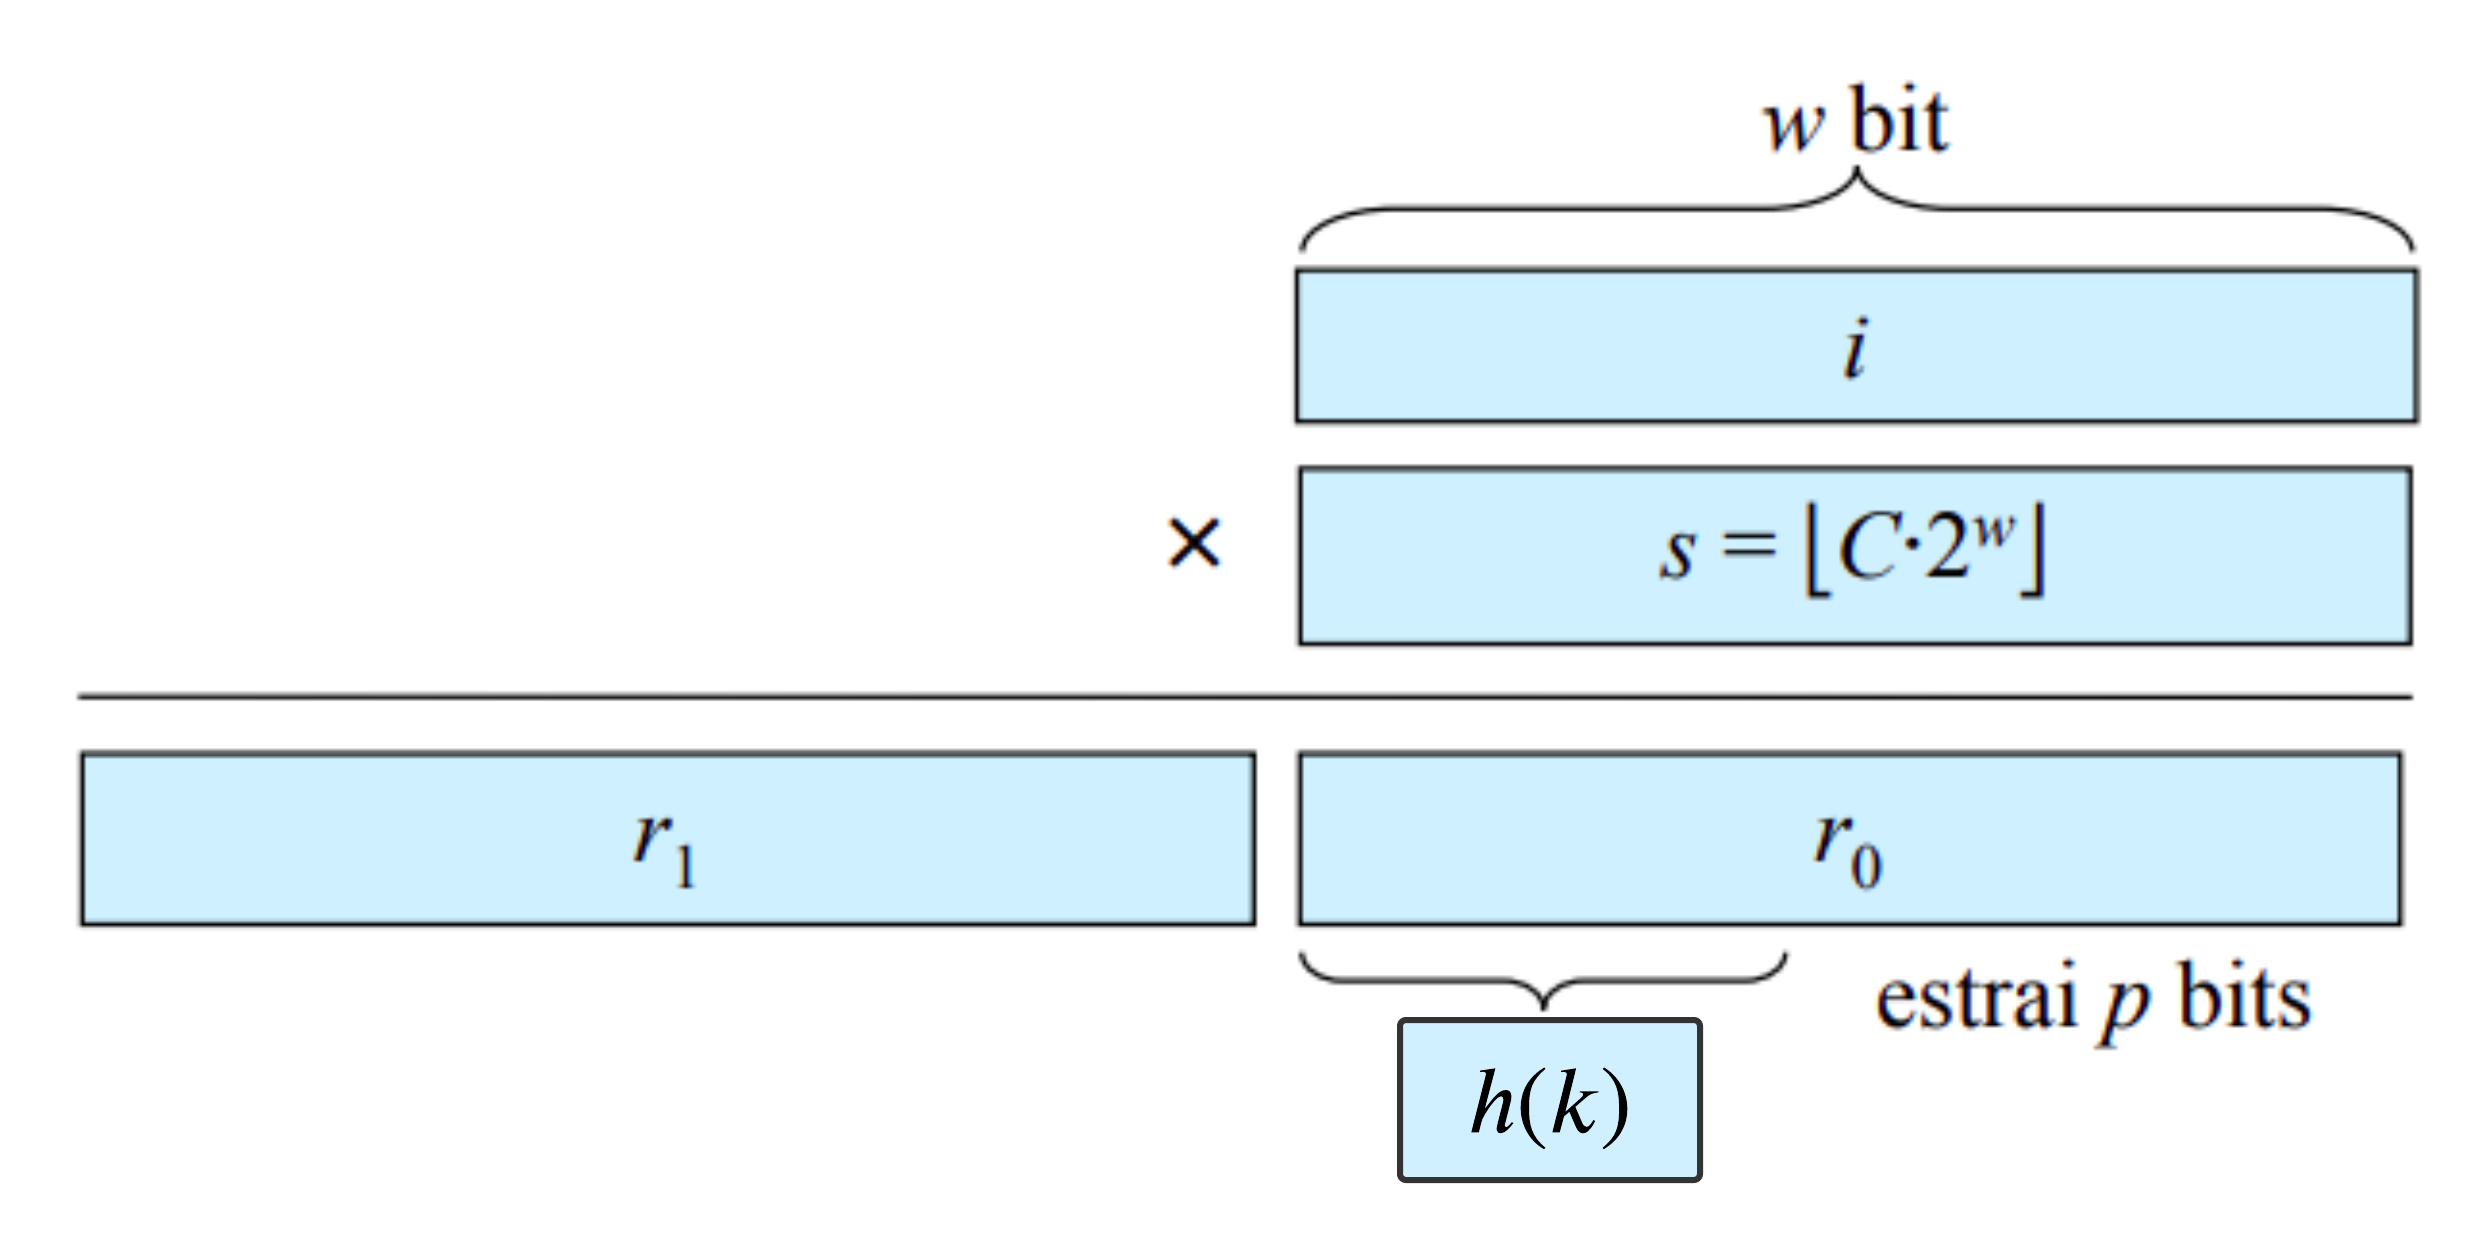
\includegraphics[width=0.8\textwidth]{metodo-moltiplicazione.png}
    \caption{Implementazione efficiente del \emph{metodo della moltiplicazione}}
\end{figure}\noindent
In definitiva, il \emph{metodo della moltiplicazione} sembra offrire una soluzione
sufficientemente efficacie anche se in realtà, la \emph{funzione hash} ottenuta non
gode di \emph{uniformità semplice} e non viene mai usata in applicazioni reali.

\section{Gestione delle collisioni}
Se abbiamo stabilito che non possiamo garantire l'assenza di \emph{collisioni}
dobbiamo definire una metodologia per la loro gestione. In particolare, se,
in fase di inserimento, la posizione in cui dovremmo inserire una chiave è
già occupata, dovremo trovarne una alternativa e, allo stesso modo, se in fase di
ricerca la chiave cercata non è nella posizione attesa, dovremo cercarla
altrove. Questa ricerca dovrebbe costare $O(1)$ nel caso medio e $O(n)$ nel caso
pessimo.

Le tecniche possibili sono due: \emph{liste di trabocco} e \emph{indirizzamento
aperto}. Queste due sono anche chiamate rispettivamente tecniche a
\emph{memorizzazione esterna} e \emph{interna}.

\subsection{Liste di trabocco}
Questa metodologia prevede che tutte le chiavi con lo stesso \emph{hash}
vengano memorizzate in una \emph{lista monodirezionale} o in un \emph{vettore
dinamico}. Ogni cella della \emph{tabella hash} poi conterrà un puntatore alla
testa della \emph{lista} o al primo elemento del \emph{vettore} associato a quella
posizione.

\begin{figure}[h!]
    \centering
    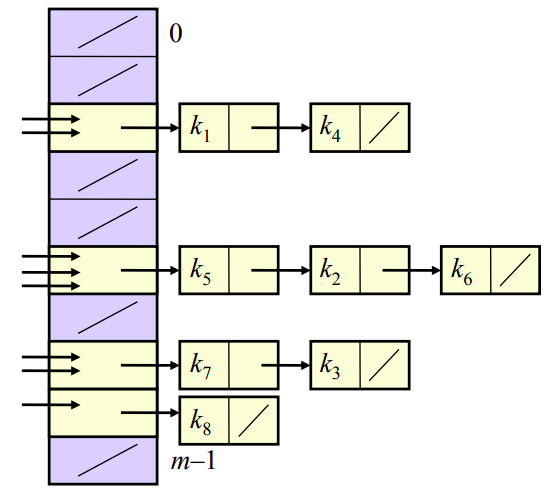
\includegraphics[width=0.6\textwidth]{liste-di-trabocco1.png}
    \caption{Struttura di una \emph{tabella hash} con \emph{liste di trabocco}}
\end{figure}\noindent
La funzione \texttt{insert()} va ad aggiungere in testa la chiave, mentre la
\texttt{lookup()} e la \texttt{remove()} scansionano la \emph{lista} fino
a trovare la chiave cercata.

\paragraph{Complessità}
Per studiare la \emph{complessità} di questa soluzione abbiamo bisogno di
definire alcuni parametri:
\begin{itemize}
    \item $n$: numero di chiavi memorizzate nella \emph{tabella hash};
    \item $m$: dimensione della \emph{tabella hash};
    \item $\alpha=\frac{n}{m}$: \emph{fattore di carico} della \emph{tabella hash};
    \item $I(\alpha)$: numero medio di accessi per la ricerca di una chiave che
    non è presente nella \emph{tabella hash} (ricerca con insuccesso);
    \item $S(\alpha)$: numero medio di accessi per la ricerca di una chiave che
    è presente nella \emph{tabella hash} (ricerca con successo);
\end{itemize}\noindent
Ovviamente il caso pessimo è quello in cui $m=1$ e quindi tutte le chiavi sono
inserite in un'unica lista e quindi la \emph{complessità} è pari a quella che
si avrebbe in un \emph{dizionario} implementato come \emph{vettore non ordinato} o
come \emph{lista}.

\bigskip\noindent
Studiare il caso medio invece, ci richiede di fare delle assunzioni. In particolare,
ipotizziamo che la \emph{funzione hash} costi $\Theta(1)$ e che consenta un
\emph{hashing uniforme}. Fatte queste ipotesi, ci aspettiamo che ogni
\emph{lista}/\emph{vettore} abbia una lunghezza pari ad $\alpha=\frac{n}{m}$.

In una ricerca con insuccesso devono ovviamente essere toccati tutti i valori di
una lista, mentre nelle ricerche con successo, in media, ne vengono toccati la
metà. Questo, unito al fatto che calcolare la posizione di ricerca costa
$\Theta(1)$, ci porta ad avere, rispettivamente, un costo $\Theta(1)+\alpha$ e
$\Theta(1)+\frac{\alpha}{2}$ per le ricerche con insuccesso e con successo.

\bigskip\noindent
Ma qual è il significato del \emph{fattore di carico}?

Il parametro influenza il costo delle operazioni sulla \emph{tabella hash}.
Per esempio, se $n=O(m)$, $\alpha=O(1)$ e quindi tutte le operazioni costano $O(1)$.

\subsection{Indirizzamento aperto}
Il problema delle \emph{liste di trabocco} è che ci costringono a
realizzare una \emph{struttura dati} complessa. L'idea alla base delle
implementazioni a \emph{indirizzamento aperto} invece, è di memorizzare tutte le
chiavi nella \emph{tabella stessa} in modo tale che ogni posizione contenga
una chiave, oppure \texttt{nil}.

Quindi, se in fase di inserimento la posizione calcolata è già
occupata, se ne sceglie un'altra. Per la ricerca invece, si parte dalla posizione
prescelta e si visitano tutte le posizioni alternative fino a quando non si
trova la chiave cercata. Per affrontare nel dettaglia questa tecnica implementativa
diamo alcune definizioni:
\begin{definition}[Ispezione]
    Un'ispezione è l'esame di una posizione durante la ricerca.
\end{definition}\noindent
Ovviamente, il numero massimo di ispezioni coincide con la dimensione $m$ della
\emph{tabella hash}. Modifichiamo la definizione di \emph{funzione hash} in modo
da includere il concetto di \emph{ispezione}.
\begin{definition}[Funzione hash per tabelle ad indirizzamento aperto]
    In una tabella hash implementata con la tecnica dell'indirizzamento aperto,
    la funzione hash $H$ è definita come
    \[H:\mathcal{U}\times\overbrace{\{0,\,\dots,\,m-1\}}^{\text{Numero di ispezione}}
    \to\overbrace{\{0,\,\dots,\,m-1\}}^{\text{Posizione nella tabella}}\]
\end{definition}
\begin{definition}[Sequenza di ispezione]
    Una sequenza di ispezione $[H(k,0),\,H(k,1),\,\dots,\,H(k,m-1)]$ è una
    permutazione degli indici $[0,\,\dots,\,m-1]$ corrispondente all'ordine
    in cui vengono visitate le posizioni della tabella.
\end{definition}\noindent
Generalmente non dovrebbe servire visitare tutte le posizioni, ma in ogni caso,
vogliamo evitare di visitarne più volte la stessa.

\begin{figure}[ht]
    \centering
    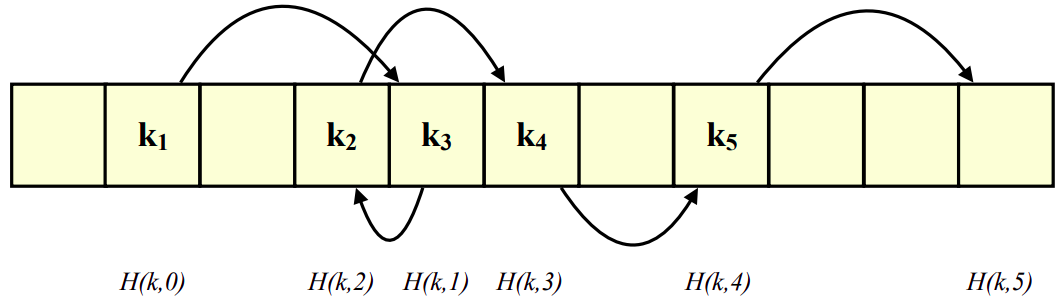
\includegraphics[width=\textwidth]{sequenza-ispezione-1.png}
    \caption{Esempio di \emph{sequenza di ispezione}}
\end{figure}

\newpage\noindent Ma cosa succede al \emph{fattore di carico}?

Siccome $0\leq n\leq m$, anche $\alpha$ è compreso tra 0 e 1 (estremi inclusi).
Questo comporta che la \emph{tabella hash} potrebbe andare in overflow,
ovvero occupare tutte le posizioni.

\bigskip\noindent
Generalizzando il concetto di \emph{uniformità semplice}, diamo la definizione di
\emph{hashing uniforme}.
\begin{definition}[Hashing uniforme]
    Si parla di hashing uniforme quando una chiave ha la stessa probabilità di
    avere come sequenza di ispezione una qualsiasi delle $m!$ permutazioni di
    $[0,\,\dots,\,m-1]$.
\end{definition}\noindent
Nella realtà è difficile raggiungere l'\emph{hashing uniforme}, per cui ci si
accontenta di ottenere alcune delle possibili permutazioni.

Le \emph{sequenze di ispezione} dipendono dalla tecnica di ispezione che si usa e
le più diffuse sono: \emph{ispezione lineare}, \emph{quadratica} e
\emph{doppio hashing}.

\paragraph{Ispezione lineare}
Questa tecnica definisce la \emph{funzione hash} come:
\[H(k,i)=(H_1(k)+h\cdot i)\Mod{m}\]
In questa definizione, $h$ è il passo della sequenza e di conseguenza la
\emph{sequenza di ispezione} per una chiave $k$ diventa:
$[H_1(k),\,H_1(k)+h,\,H_1(k)+2h,\,\dots]$.

Questa tecnica ci permette di avere al massimo $m$ possibili \emph{sequenze} che
sono tutte determinabili dalla posizione della prima \emph{ispezione}. Inoltre,
c'è il problema della cosiddetta \emph{aggregazione primaria} (o \emph{primary
clustering}) che comporta la formazione di sotto sequenze sempre più lunghe di
posizioni occupate, col risultato che una posizione libera preceduta da $i$
posizione occupate viene riempita con probabilità $\frac{i+1}{m}$ e i tempi di
inserimento e cancellazione crescono sempre di più.

\paragraph{Ispezione quadratica}
L'\emph{ispezione quadratica} segue lo stesso principio di quella \emph{lineare},
ma le \emph{ispezioni} hanno un offset che dipende da una funzione quadratica del
numero di \emph{ispezione}. La \emph{funzione hash} è infatti definita come:
\[H(k,i)=(H_1(k)+h\cdot i^2)\Mod{m}\]
Anche in questo caso sono possibili $m$ \emph{sequenze di ispezione}, ma nessuna
di esse è una permutazione e si propone il problema dell'\emph{aggregazione
secondaria} (o \emph{secondary clustering}) ovvero, chiavi con
la stessa posizione iniziale hanno anche \emph{sequenze di ispezione} identiche.

\paragraph{Doppio hashing}
In questo caso $H$ è:
\[H(k,i)=(H_1(k)+i\cdot H_2(k))\Mod{m}\]
dove $H_1(k)$ fornisce la posizione iniziale e $H_2(k)$ l'offset per le
successive \emph{ispezioni}. Sono possibili $m^2$ \emph{sequenze}, ma per
garantire una permutazione completa $H_2(k)$ deve essere coprimo con $H_1(k)$.
Cioè, se $m=2^p$, $H_2(k)$ deve essere un numero dispari, mentre se $m$ è
primo, $H_2(k)$ deve essere un valore minore di $m$.

\begin{minicode}{Implementazione tabella hash con hashing doppio}
\bc{ITEM}[] K\hfill\com{Tabella delle chiavi}
\bc{ITEM}[] V\hfill\com{Tabella dei valori}
\bc{int} m\hfill\com{Dimensione della \emph{tabella hash}}

\nl\ind\bc{HASH} Hash(\bc{int} dim)\\
    \bc{HASH} t = new \bc{HASH}\\
    t.m = dim\\
    t.K = new \bc{ITEM}[dim]\\
    t.V = new \bc{ITEM}[dim]\\
    \indf for (i = 0 to dim - 1) do\\
        t.K[i] = nil\\
    \indf return t

\nl\com{Cerca la posizione associata ad una chiave}
\rmbreak\ind\bc{int} scan(\bc{ITEM} k, \bc{boolean} insert)\\
    \bc{int} delpos = m\hfill\com{Prima posizione deleted}
    \bc{i} = 0\hfill\com{Numero di \emph{ispezione}}
    \bc{j} = H(k)\hfill\com{Posizione di partenza}
    \indf while (K[i] $\neq$ k and K[j] $\neq$ nil and i < m) do\\
        \indff if (K[j] == deleted and delpos == m) then\\
            delpos = j\\
        \indff j = (j + H'(k)) mod m\\
        \indff i = i + 1\\
    \indf if (insert and K[j] $\neq$ k and delpos < m) then\\
        return delpos\\
    \indf return j

\nl\com{Cerca e restituisce il valore associato a una chiave oppure nil}
\rmbreak\ind\bc{ITEM} lookup(\bc{ITEM} k)\\
    \bc{int} i = scan(k, false)\\
    \indf if (k[i] == k) then\\
        return V[i]\\
    \indf else\\
        return nil
\end{minicode}
\newpage
\begin{codecont}
\com{Inserisce un'associazione chiave-valore o ne modifica il valore associato}
\rmbreak\ind insert(\bc{ITEM} k, \bc{ITEM} v)\\
    \bc{int} i = scan(k, true)\\
    if (K[i] == nil or K[i] == deleted or K[i] == k) then\\
        \indf k[i] = k\hfill\com{È inutile se K[i] == k}
        \indf V[i] = v\\
    \ind else\\
        \indf \{ Errore:\,la tabella è piena \}

\nl\com{Rimuove un'associazione chiave-valore}
\rmbreak\ind remove(\bc{ITEM} k)\\
    \ind \bc{int} i = scan(k, false)\\
    \ind if (K[i] == k) then\\
        \indf K[i] = deleted\\
        \indf V[i] = nil\\
\end{codecont}

\bigskip\noindent
Esaminiamo più nel dettaglio la funzione \texttt{scan()}. Può infatti risultare
strano il fatto che abbiamo introdotto il valore \texttt{deleted} che usiamo al
posto di \texttt{nil} per marcare una posizione come libera dopo una cancellazione.
Questo serve a evitare situazioni come quella in figura, in cui la ricerca della
chiave $k_5$ si interrompe all'\emph{ispezione} della posizione \texttt{nil}
facendo erroneamente credere che $k_5$ non sia presente nella \emph{tabella hash}.

\begin{figure}[h!]
    \centering
    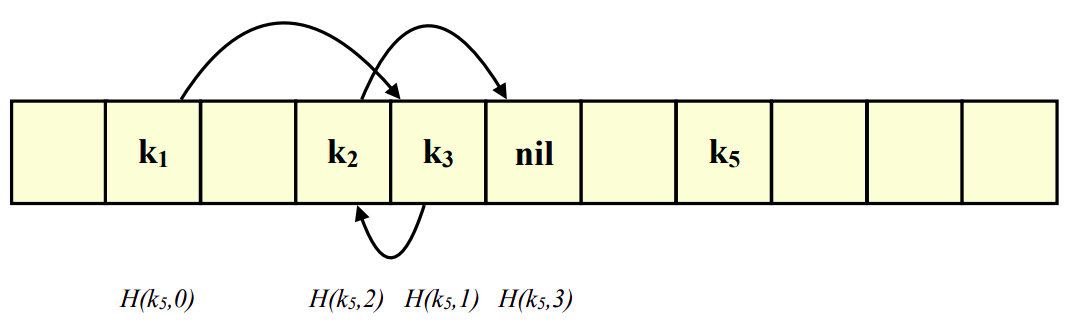
\includegraphics[width=\textwidth]{sequenza-ispezione-2.png}
    \caption{\emph{Sequenza di inspezione} errata}
\end{figure}\noindent
L'utilizzo del valore \texttt{deleted} al posto di \texttt{nil} ci consente di
marcare le posizioni nelle quali in precedenza c'era un valore che poi è stato
eliminato. In particolare, le posizioni \texttt{deleted} sono considerate come
piene in fase di ricerca e vuote in fase di inserimento.

Questa soluzione risolve il problema della ricerca, ma rende il tempo di ricerca
non più dipendente dal \emph{fattore di carico} $\alpha$ e fa sì che il
concatenamento sia più comune nelle implementazioni che ammettono la rimozione.

\newpage
\subsection{Complessità delle diverse implementazioni}
Mettiamo a confronto le \emph{complessità} di alcune delle implementazioni viste:
\begin{table}[ht]
    \renewcommand{\arraystretch}{1.5}
    \centering
    \begin{tabular}{|l|c|c|c|}
        \hline
        \textbf{Tecnica} & \bm{$\alpha$} & \bm{$I(\alpha)$} & \bm{$S(\alpha)$}\\
        \hline
        Lineare & $0\leq\alpha<1$ & $\frac{(1-\alpha)^2+1}{2(1-\alpha)^2}$ &
        $\frac{1-\frac{\alpha}{2}}{1-\alpha}$\\
        \hline
        Hashing doppio & $0\leq\alpha<1$ & $\frac{1}{1-\alpha}$ &
        $-\frac{1}{\alpha}\ln(1-\alpha)$\\
        \hline
        Liste di trabocco & $\alpha\geq0$ & $1+\alpha$ & $1+\frac{\alpha}{2}$\\
        \hline
    \end{tabular}
\end{table}
\begin{figure}[ht!]
    \centering
    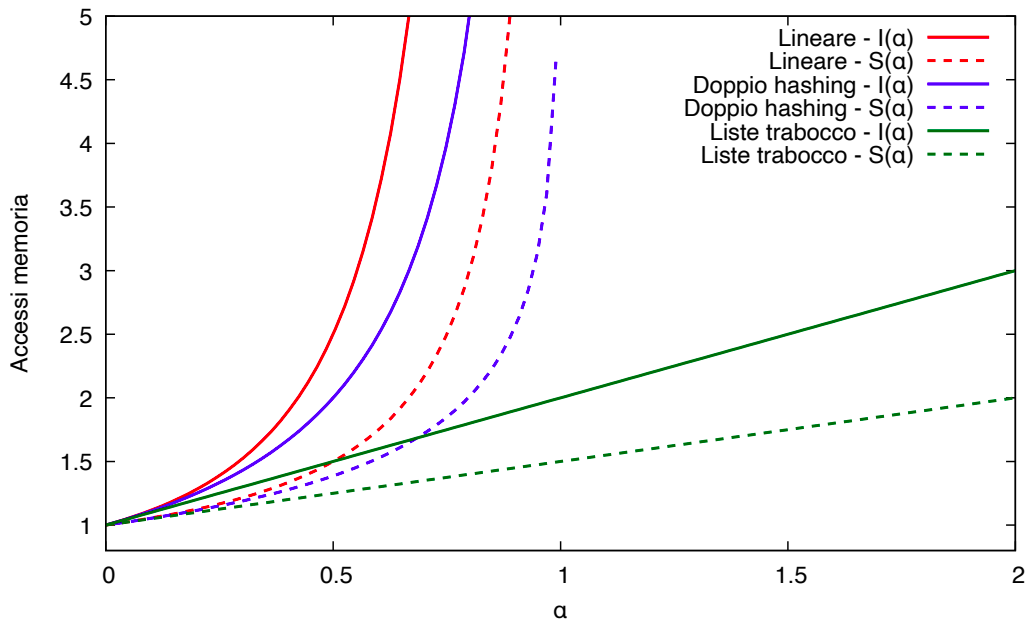
\includegraphics[width=\textwidth]{complessita-hash-table.png}
    \caption{\emph{Complessità} delle \emph{tabelle hash} a confronto}
\end{figure}

\paragraph{Conclusioni}
Per concludere possiamo dire che le \emph{tabelle hash} permettono di implementare
in modo molto efficiente dei \emph{dizionari}, ma hanno una scarsa \q{locality
of reference} che genera molte \emph{cache miss} e inoltre, non permettono di
ordinare le chiavi.